\chapter{Comparison}
\label{chapter:comparison}

After finishing the prototype of the plug-in comparison of the main functionality with the equivalent from Waves was performed to find out how likely the results can get with fitting parameters at the prototype version of the implemented gain adaption and also to evaluate the flexibility of the study plug-in and to gather thoughts about how to set own parameters and constants later on.\\

\section{How}

It is expected that it would not be effective to try different picks for the parameters manually and compare the outcomes as there are at least several parameters which can be adjusted to result in a lot of combinations. Therefore, this task is transferred to the computer program.\\
The scipy.optimize package for Python deals with optimisation tasks for example the algorithmic minimisation of a problem according to the result of a self defined function (see chapter \ref{chapter:basics}.3).\\
Therefore a function to compare the resulting audio files after processed with the “Vocal Rider” and the study plug-in was developed. The resulting algorithm returns a value describing the deviation.\\
Through the optimisation process the parameter adjustments of the “Vocal Rider” differed between attempts but stayed constant in the process. The parameters of the study plug-in were changed continuously to achieve a preferably small deviation.\\

\section{Circumstances}

In order to let the optimisation algorithm amend different parts of the study plug-in, $L_{goal}$, RMS time, compress time, amplification time, gate threshold and lookahead delay are defined as variables. At start guessed values for each of the parameters are chosen and stored in an array which was altered through optimisation process and fed into the deviation function at every step of it.\\
For quantification of the deviation for the current parameter array the function sums up the squared difference between both resulting audio files for every sample. The result from the “Vocal Rider” was created in the DAW Pro Tools 11. The study implementation is called in the deviation function with the current parameter array.\\
When the optimisation search was done the outcome was fed into another function which displays the gain adaption from each plug-in in a collective graph. This gives a great overview of the result and remaining diversion of the implementations.\\

\section{Approaches}

Algorithmically the optimisation procedure tests small variations in the parameter array and watches the outcome. If the initial values were not set well, the differences calculated by the comparison function are small and the scipy.optimize.minimize algorithm did not know were to continue the search. With an unfavorable parameter set the gain curves are dissimilar and small variations might find a local minima in diversion but not the solution expected.\\
To obtain a good initial guess the scipy.optimize.brute method (see chapter\ref{chapter:basics}.3) was used. As just an approximation to the final solution was required large step sizes suiting the different ranges were set. Therefore the scipy.optimize.brute algorithm just had to deal with three to six possibilities per parameter.\\
The best initial values were fed into scipy.optimize.minimize. With good initialisation this method returned useful results meaning parameter arrays with likely outcome to the Waves plug-in. However the graphical representation of the 'Vocal Rider' gain adaption was not as expected: some gain values were jumping out of the line for single samples. After testing possible causes this could be explained by rounding errors of the DAW on export of audio files. While this error was unproblematic at most points in time it became visible with values near zero. Such small values could easily be doubled or increased even further by the errors which consequently affected the calculation of the local gain. At first this was solved this with a gate for small samples at gain calculation. Afterwards it got fixed anyhow as the algorithm was changed to use RMS averages for displaying the graphical evaluation.\\

\begin{figure}[H]
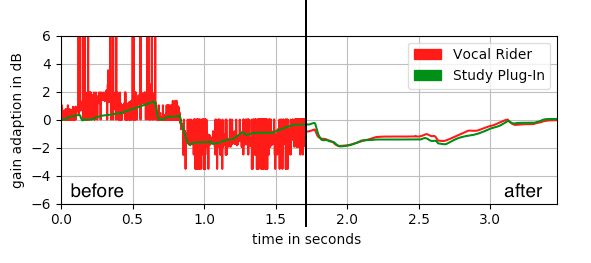
\includegraphics[width=\textwidth]{images/afterSmooth}
\caption{Optimisation result with (left) and w/o (right) rounding errrors}
\end{figure}

The behaviour of both plug-ins was compared by testing with optimised parameters on different vocal tracks in various length. The gain range of both plug-ins was set to +/- 6dB. The \textit{target} threshold of the “Vocal Rider” was adjusted to a reasonable value for all test files. The default and live component of the Vocal Rider were used. Additionally the plug-in from Waves wrote a gain automation and it read it through the export process for a further test file.\\

\section{Results}

The differences between the default “Vocal Rider” component, the live version and the self-automated were negligible. The automated plug-in provided in the same result as the default. It did not adapt for every sample but frequently after small consistent time steps, probably derivable from the communication between DAW and plug-in. The live version created no critical difference to the default - as it could be expected. It just added a potentiometer to adjust the noise gate for live performances. Therefore, in tests further described results will always relate to the default plug-in version.\\
The first analysis result was that the Waves plug-in is not using a lookahead and consequently the parameter optimisation always resulted in a lookahead value of 0ms. This was to expect for the live component but not necessary for its standard use, as today's DAWs can easily compensate the produced delay. Obviously it was not considered as important by the authors in contrast to the plug-in design in this study as explained in section 3.7.\\
The second analysis result was that the Waves plug-in does not start fading to 0dB gain immedietly when it detects no vocal signal but only after several milliseconds of idle time, in contrast to the study plug-in's prototype. This feature was assumed to enables the plug-in to ignore small gaps in the vocals when the singer is breathing or doing a rhythmic break where a smoothed gain reset to 0dB is not necessary and can even be counterproductive (as the gain adaption needs a few milliseconds). Therefore it resulted in the implementation of a similar function for the study plug-in as it was assumed to work even better in combination with a small lookahead (see chapter \ref{chapter:improvements}.4).\\
Despite the described obvious conceptual differences the optimisation algorithm was able to bring both plug-ins to quite close results in terms of the gain adaption. The “Vocal Rider” seems to need a short time (about one second) to adjust its behaviour. This presumption resulted from different tests where both plug-ins were operating quite similar except for the first second. As a consequence the compare function was improved by ignoring the first second of the result.\\
Initially the study plug-in was able to imitate a section of the “Vocal Rider”s gain adaption for test files of longer duration, but not to imitate the gain adaption for the whole signal. Therefore causes for this behaviour were evaluated taken into account that the amplification of the “Vocal Rider” with slow attack time results in greater gain alteration than the compression of it with very fast attack time. It seemed as if compression was attenuated while amplification was not. The weakened compression reminded of standard compressor behaviour. Therefore an additional ratio parameter was implemented for the Python test version of the plug-in. This parameter reduces the value of the calculated gain adaption before it is smoothed and applied. Subsequently the new parameter was added to the parameter array for the optimisation algorithm. Simultaneously, the lookahead optimisation was removed as it always resulted in 0ms. The extended optimisation validated the assumption described above and got both gain curves close together for the whole test files.\\
\begin{figure}
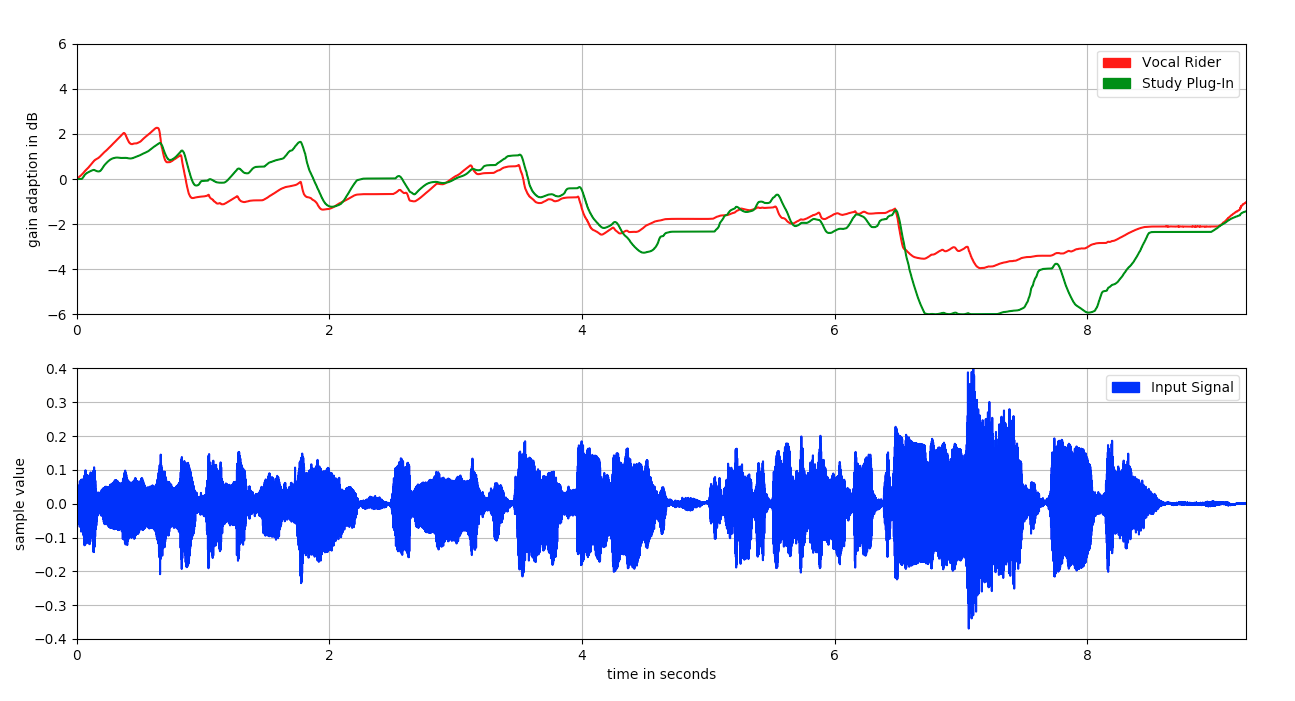
\includegraphics[width=\textwidth]{images/onlyParts}
\caption{Gain Reduction comparison with interim optimisation result}
\end{figure}
In conclusion it can be stated that the “Vocal Rider” does gain adaption on the decreasing part quite similar to a compressor but without any colouring of the altered signal and a small ratio\footnote{proportion between increment of input and output signal above the threshold}. The study plug-in was able to get a similar result with a compress time of barely 100ms and a additional gain factor of 2/3 (1/3 slope\footnote{slope $= 1 - 1/$ratio}) before smoothing. In terms of amplification of the input the plug-in by Waves takes a comparatively long time period. It takes a attack time of about 2,4s for the study plug-in to imitate its performance. The gate threshold-to-$L_{goal}$ relation of the study plug-in seems to fit the working method of the second test subject.\\
The comparison of the two plug-ins extended the main idea about some additional features and got some progress on the final set of the parameters to get to the main objective. Even though the results of the analysis of the “Vocal Rider” is not fitting the initial model of the study plug-in in all terms it still corroborated present work and leads to useful ideas.\\

\begin{figure}
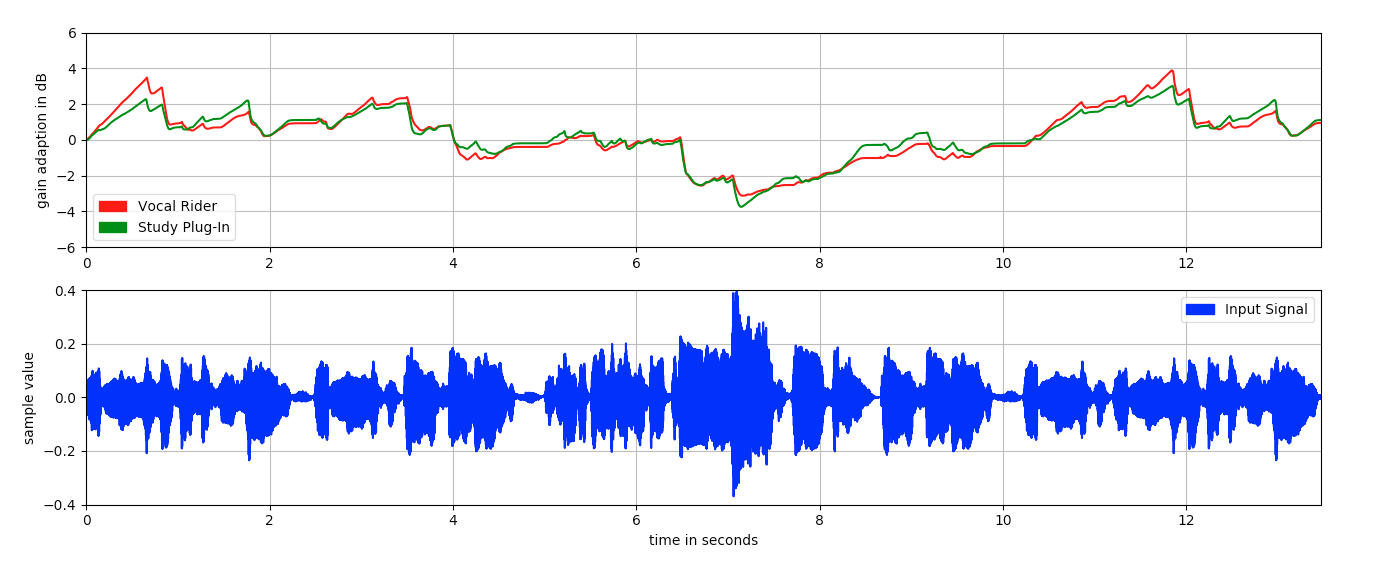
\includegraphics[width=\textwidth]{images/compareResult}
\caption{Gain Reduction comparison with final optimisation result}
\end{figure}